\section{Filter}


\subsection{Grundtypen}{291}

Filter sind mehrheitlich \textbf{frequenzselektive, lineare Netzwerke}, welche gewisse Frequenzbereiche übertragen
und andere dämpfen. Die fünf \textbf{frequenzselektiven Grundtypen} sind: 

\begin{minipage}[t]{0.25\columnwidth}
    \begin{itemize}
        \item Tiefpass (TP)
        \item Hochpass (HP)
    \end{itemize}
\end{minipage}
\hfill
\begin{minipage}[t]{0.35\columnwidth}
    \begin{itemize}
        \item Bandpass (BP)
        \item Bandsperre, Notch (BS)
    \end{itemize}
\end{minipage}
\hfill
\begin{minipage}[t]{0.25\columnwidth}
    \begin{itemize}
        \item Allpass
    \end{itemize}
\end{minipage}


\subsection[Frequenzgang H(jimg omega) -- Übertragungsfunktion H(s)]{Frequenzgang $H(\jimg \omega)$ -- Übertragungsfunktion $H(s)$}{294}

Für den Frequenzgang $H(\jimg \omega)$ und die Übertragungsfunktion $H(s)$ gelten die folgenden Zusammenhänge

$$ | H(\jimg \omega) |^2 = H(\jimg \omega) \cdot H^*(\jimg \omega) = H(\jimg \omega) \cdot H(- \jimg \omega) = H(s) \cdot H(-s) \Big|_{s = \jimg \omega} $$
$$ H(s) \cdot H(-s) = | H(\jimg \omega) |^2 \Big|_{\omega^2 = -s^2} $$
\textbf{Hinweis:} $| H(\jimg \omega) |^2$ ist immer eine Funktion in $\omega^2$, da der Amplitudengang eine gerade Funktion ist!

\vspace{0.2cm}

Da in der Praxis \textbf{jeweils nur $\bm{H(s)}$ interessant} ist, muss $H(s)$ aus $| H(\jimg \omega) |^2$ 'isoliert' werden. 
Dies ist durch den folgenden Zusammenhang möglich.

$$ \boxed{ \underbrace{ \frac{N(s)}{D(s)} }_{H(s)} \cdot  \underbrace{ \frac{N(-s)}{D(-s)} }_{H(-s)} = | H(\jimg \omega) |^2 \Big|_{\omega^2 = -s^2} } $$
\textbf{Hinweis:} $D(s)$ muss aus Stabilitätsgründen ein Hurwitz-Polynom sein!


\subsection{Approximation im Frequenzbereich}

Die wichtigste Aufgabe der Filtertheorie ist die \textbf{Bestimmung der Übertragungsfunktion, die einen vorgegebenen 
Frequenzgang gewährleistet.} Zuerst soll der \textbf{Amplitudengang} $| H(\jimg \omega) |$ im Frequenzbereich approximiert werden.
Der vorgeschriebene Phasengang wird dann allenfalls mit zusätzlichen Allpass-Filtern erreicht. 


\subsubsection{Toleranzschema (Stempel und Matritze) -- Filterspezifikation}
\label{Toleranzschema}

\begin{minipage}[c]{0.48\columnwidth}
    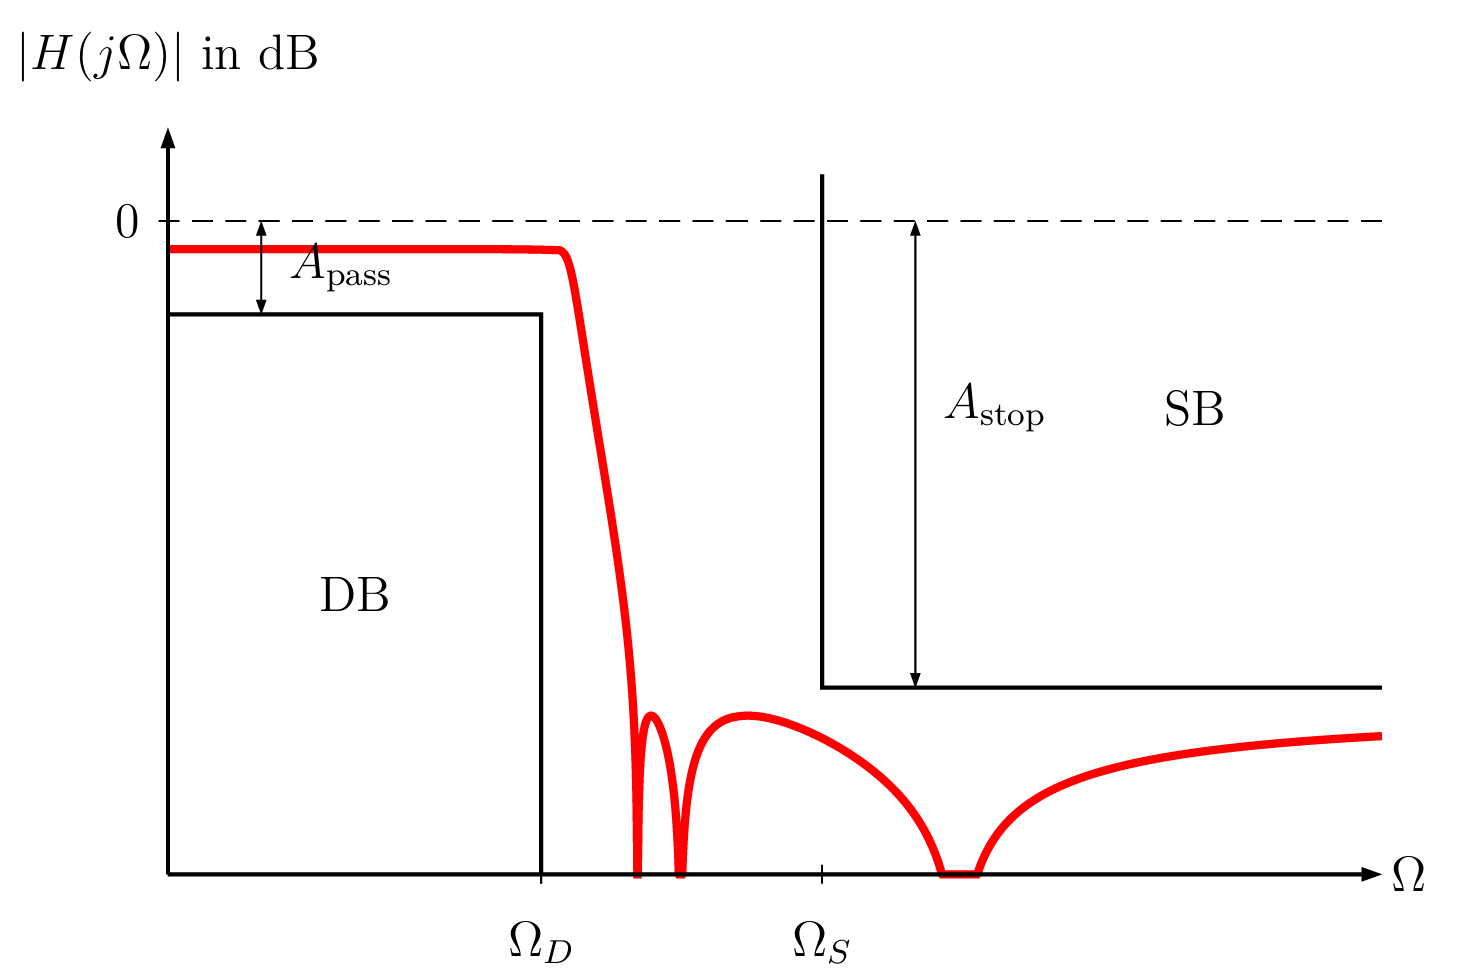
\includegraphics[width=\columnwidth]{images/filter_toleranzschema.png}
\end{minipage}
\hfill
\begin{minipage}[c]{0.48\columnwidth}
    Die Anforderungen an ein Filter werden häufig im \textbf{Toleranzschema beschrieben}. Dieses steht jeweils 'auf dem Kopf'.

    \begin{itemize}
        \item Im \textbf{Durchlassbereich (DB)} bestimmt der Stempel die maximal zulässige \textbf{Dämpfung} $A_{\rm max}$
        \item Im \textbf{Sperrbereich (SB)} bestimmt die Matritze die minimal nötige \textbf{Dämpfung} $A_{\rm min}$
    \end{itemize}
\end{minipage}

$$\boxed{ A_{\deci \bel}(\omega) = 10 \cdot \log \Biggl( \frac{1}{|H(\omega)|^2} \Biggr) = - 20 \cdot \log \bigl(|H(\omega)| \bigr) 
    \quad \textrightarrow\ \text{Dämpfung!} } $$


\subsubsection{Frequenznormierung}
\label{Frequenznormierung}
 
Um möglist kompakte \textbf{Tabellen} zu haben, wird auf Frequenzen normiert. Grundsätzlich kann auf eine beliebige Frequenz normiert
werden. Allerdings gilt grundsätzlich:

\begin{itemize}
    \item \textbf{HP / TP:} Normierung bezüglich \textbf{Grenzfrequenz} des Durchlassbereichs $\omega_r = \omega_D$
    \item BP / BS: Normierung bezüglich der Mittenfrequenz $\omega_r = \omega_m$
\end{itemize}
\vspace{0.2cm}

\begin{minipage}[c]{0.48\columnwidth}
    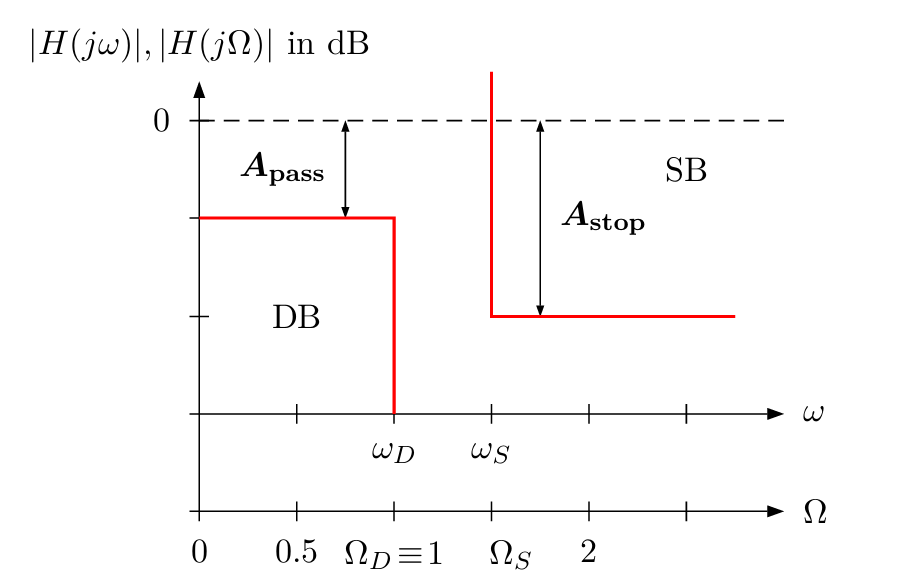
\includegraphics[width=\columnwidth]{images/filter_toleranzschema_frequenznormierung.png}
\end{minipage}
\hfill
\begin{minipage}[c]{0.48\columnwidth}
    \begin{center}
       \textbf{\myul{Normierte Grössen}}  
    \end{center}

    \vspace{-0.3cm}
    \begin{minipage}[c]{0.3\columnwidth}
        $$ \boxed{ S = \frac{s}{\omega_r}} $$
    \end{minipage}
    \hfill
    \begin{minipage}[c]{0.3\columnwidth}
        $$ \boxed{ \Omega = \frac{\omega}{\omega_r}} $$
    \end{minipage}
    \hfill
    \begin{minipage}[c]{0.3\columnwidth}
        $$ \boxed{ \sigma' = \frac{\sigma}{\omega_r}} $$ 
    \end{minipage}

    \vspace{0.2cm}
    \textbf{Entnormierung:} Jeweils $S$ in der normierten Funktion durch $\frac{s}{\omega_r}$ ersetzen.
\end{minipage}


\subsection{Ideales Tiefpassfilter}{297}

\begin{minipage}[c]{0.48\columnwidth}
    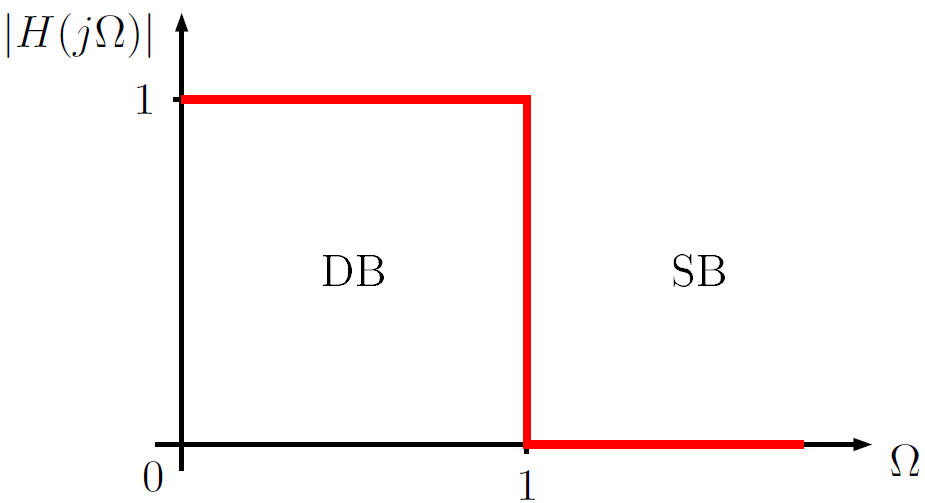
\includegraphics[width=\columnwidth]{images/filter_toleranzschema_idealer_tiefpass.png}

    \begin{itemize}
        \item DB: keine Dämpfung
        \item SB: kein Ausgangssignal
    \end{itemize}
\end{minipage}
\hfill
\begin{minipage}[c]{0.42\columnwidth}
    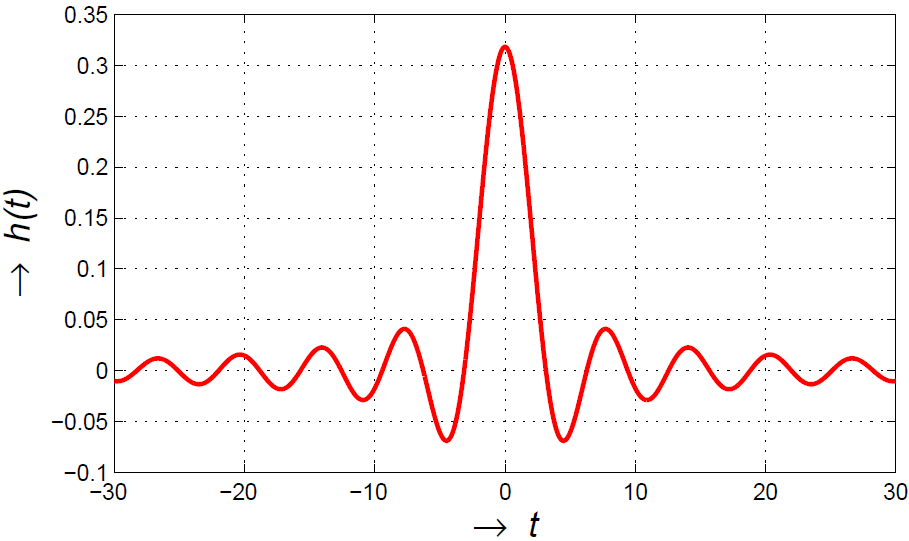
\includegraphics[width=\columnwidth]{images/filter_impulsantwort_idealer_tiefpass.png}
    
    \begin{itemize}
        \item Akausale Impulsantwort $h(t)$
    \end{itemize}
\end{minipage}

\vspace{0.2cm}
\textrightarrow\ Ideales Tiefpass ist physikatisch nicht realisierbar. \textrightarrow\ \textbf{Approximationen}


\subsection[Amplitudengang mit char. Funktion K(Omega2)]{Amplitudengang mit char. Funktion $K(\Omega^2)$}
\label{Amplitudengang mit char. Funktion}

Um Wurzelausdrücke zu vermeiden, wird der folgenden Ansatz verwendet
$$ \boxed{ | H(\jimg \Omega) |^2 = \frac{1}{1 + K(\Omega^2)}} $$

Im Fall des (idealen) Tiefpasses gilt für die charakteristische Funktion $K(\Omega^2)$

\begin{tabular}{l r l l}
    Durchlassbereich (DB)   & $0 \leq K(\Omega^2) \ll 1$    & für $0 \leq \Omega < 1$   & \textrightarrow\ $| H(\jimg \Omega) |^2 \approx 1$ \\
    Sperrbereich (SB)       & $K(\Omega^2) \gg 1$           & für $ \Omega > 1$         & \textrightarrow\ $| H(\jimg \Omega) |^2 \approx 0$ \\   
\end{tabular}



\subsection{Standard-Filtertypen -- Überblick}
\label{Standard-Filtertypen}

\begin{outline}
    \1 \textbf{Kritisch-gedämpfte Filter}
        \2[+] \textbf{Kein Rippel} im Durchlass- und Sperrbereich
        \2[+] Kein Überschwingen bei Impuls- und Sprungantwort
        \2[-] Braucht \textbf{hohe Ordnung} für steilen Übergang von Durchlass- zu Sperrbereich
        \2    Kaskadierung von $n$ wirkungsfreien, identischen Filtern 1. Ordnung
        \2    Bei $\Omega = 1$ \textrightarrow\ Dämpfung von $3 \, \deci \bel$
        \2    Steilheit: $- n \cdot 20 \, \deci \bel /$ Dekade
        \2    Allpolfiler: $n$ Pole am gleichen Ort in der LHE

    \1 \textbf{Butterworth}
        \2[+] \textbf{Kein Rippel} im Durchlass- und Sperrbereich
        \2[+] Im Durchlassbereich ist der Amplitudengang \textbf{maximal flach}
        \2[-] Überhöhung in der Gruppenlaufzeit der Grenzfrequenz
        \2[-] Braucht \textbf{hohe Ordnung} für steilen Übergang von Durchlass- zu Sperrbereich
        \2    Bei $\Omega = 1$ \textrightarrow\ Dämpfung von $3 \, \deci \bel$
        \2    Steilheit: $- n \cdot 20 \, \deci \bel /$ Dekade
        \2    Allpolfiler: Pole auf Einheitskreis mit Abstand $\frac{\pi}{n}$ 

    \1 \textbf{Tschebyscheff-\uproman{1}}
        \2[+] Schon für kleine Ordnungen \textbf{relativ steil} im Übergang von Durchlass- und Sperrbereich
        \2[-] \textbf{Rippel} im \textbf{Durchlassbereich} (abhängig von Ordnung $n$)
        \2[-] Keine konstante Gruppenlaufzeit (wellig)
        \2    Bei $\Omega = 1$ \textrightarrow\ Dämpfung abhängig von Rippelfaktor $e$
        \2    Steilheit: $- n \cdot 20 \, \deci \bel /$ Dekade
        \2    Allpolfiler: Pole auf einer Ellipse

    \1 \textbf{Tschebyscheff-\uproman{2}}
        \2[+] Schon für kleine Ordnungen \textbf{relativ steil} im Übergang von Durchlass- und Sperrbereich
        \2[-] \textbf{Rippel} im \textbf{Sperrbereich} (abhängig von Ordnung $n$)
        \2[-] Relativ konstante Gruppenlaufzeit
        \2    Bei $\Omega = 1$ \textrightarrow\ Dämpfung abhängig von Rippelfaktor $e$
        \2    Steilheit: $- n \cdot 20 \, \deci \bel /$ Dekade
        \2    Kein Allpolfilter

    \1 \textbf{Cauer}
        \2[+] Steilster Übergang von Durchlass- zu Sperrbereich
        \2[-] \textbf{Rippel} in \textbf{Durchlassbereich und Sperrbereich} (abhängig von Ordnung $n$)
        \2    \textbf{Kombination aus Tschebyscheff-\uproman{1} und Tschebyscheff-\uproman{2}}
        % \2    Steilheit: $- n \cdot 20 \, \deci \bel /$ Dekade
        \2    Kein Allpolfilter

    \1 \textbf{Bessel}
        \2[+] \textbf{Flachster Übergang} von Durchlass- und Sperrbereich von allen Filtern
        \2[+] Konstante Gruppenlaufzeit
        \2[-] Für steile Filter im Durchlass- und Sperrbereich nicht geeignet
        \2    Allpolfilter: Pole auf exzentrischen Kreisen in LHE
\end{outline}


\subsection{Gegenüberstellung der Filter-Approximationen} 

\scalebox{0.68}{
\begin{tabular}{|l|c|c|c|c|c|c|}
    \hline
    \multicolumn{1}{|c|}{} & \textbf{Krit. Gedämpft}                                            & \textbf{Butterworth}                                                    & \textbf{Tschebyscheff 1}                                        & \textbf{Tschebyscheff 2}                                       & \textbf{Cauer}                                                       & \textbf{Bessel}                                          \\ \hline
    \textbf{Allpolfilter}  & ja                                                                 & ja                                                                      & ja                                                              & nein                                                           & nein                                                                 & ja                                                       \\ \hline
    \textbf{Pol-Lage}      & \begin{tabular}[c]{@{}c@{}}reelle Achse\\ \textless 0\end{tabular} & \begin{tabular}[c]{@{}c@{}}Halbkreis\\ LHE\end{tabular}                 & \begin{tabular}[c]{@{}c@{}}Ellipse\\ LHE\end{tabular}           & LHE                                                            & \begin{tabular}[c]{@{}c@{}}Ellipse\\ LHE\end{tabular}                & \begin{tabular}[c]{@{}c@{}}exzentr.\\ Kreis\end{tabular} \\ \hline
    \textbf{NS-Lage}       & -                                                                  & -                                                                       & -                                                               & $\jimg \omega$-Achse                                           & $\jimg \omega$-Achse                                                 & -                                                        \\ \hline
    \textbf{DB}            & monoton                                                            & \begin{tabular}[c]{@{}c@{}}monoton\\ maximalflach\end{tabular}          & \begin{tabular}[c]{@{}c@{}}wellig\\ konst. Rippel\end{tabular}  & monoton                                                        & \begin{tabular}[c]{@{}c@{}}wellig\\ konst. Rippel\end{tabular}       & monoton                                                  \\ \hline
    \textbf{SB}            & streng                                                             & monoton                                                                 & monoton                                                         & \begin{tabular}[c]{@{}c@{}}wellig\\ konst. Rippel\end{tabular} & \begin{tabular}[c]{@{}c@{}}wellig\\ konst. Rippel\end{tabular}       & monoton                                                  \\ \hline
    \textbf{Phasengang}    & sehr gut                                                           & mittel                                                                  & schlecht                                                        & schlecht                                                       & wild                                                                 & bestmöglich                                              \\ \hline
\end{tabular}}


\subsubsection{Frequenzgänge / Lage der Pol- und Nullstellen}{334}

\begin{minipage}[c]{0.7\columnwidth}
    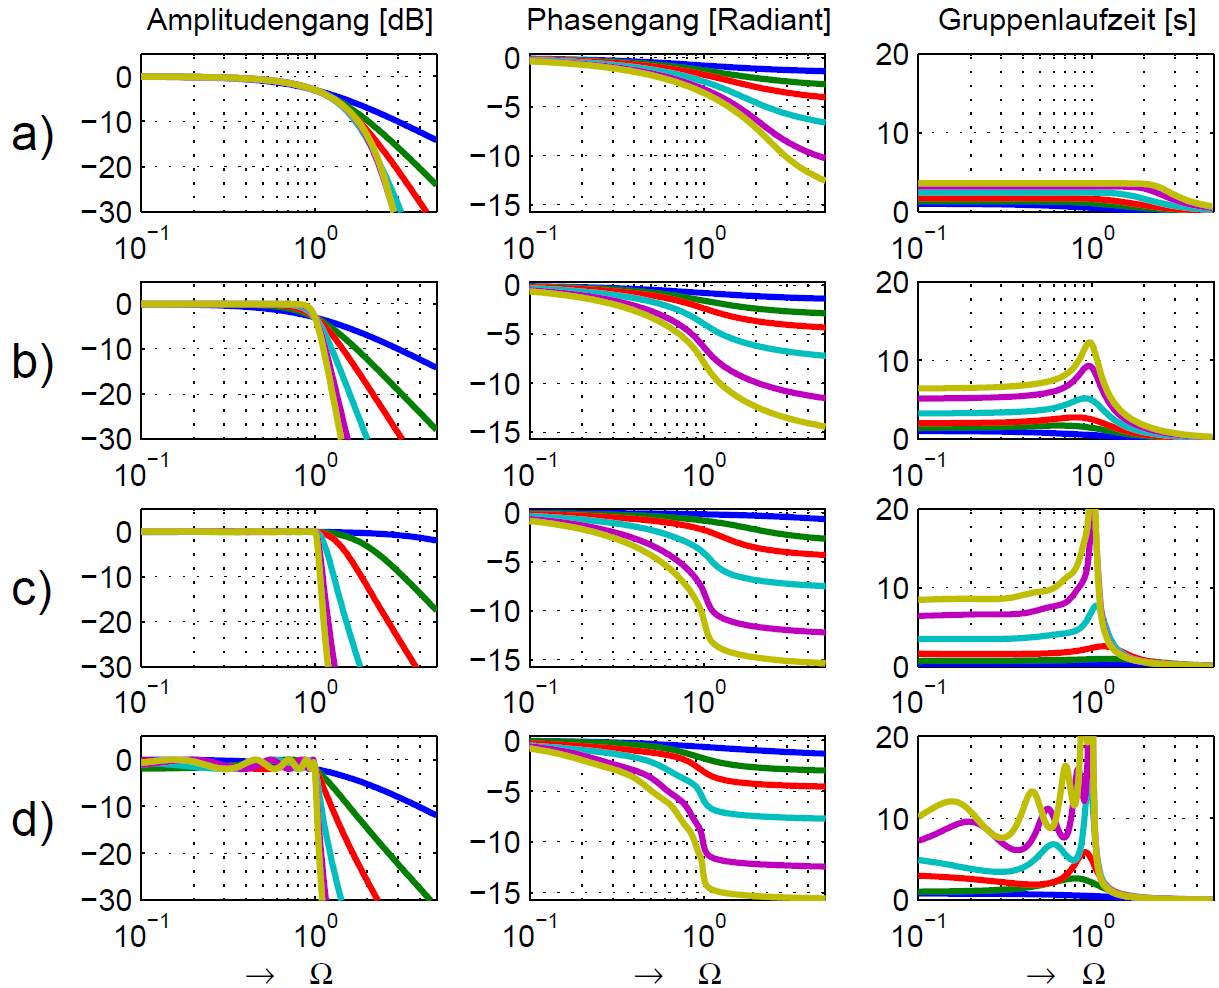
\includegraphics[width=\columnwidth]{images/filter_vergleich_frequenzgaenge.png}
\end{minipage}
\hfill
\begin{minipage}[c]{0.28\columnwidth}
    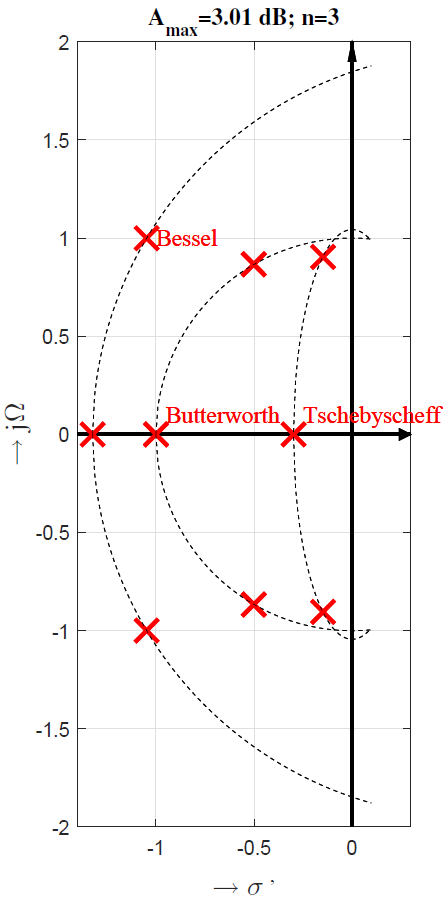
\includegraphics[width=\columnwidth]{images/filter_vergleich_pollagen.png}
\end{minipage}

\begin{tabular}{ll cc ll}
    a) & Bessel         & & & c) & Tschebyscheff ($0.1 \, \deci \bel$) \\
    b) & Butterworth    & & & d) & Tschebyscheff ($2 \, \deci \bel$) \\
\end{tabular}


\subsection{Vorgehen Filter dimensionieren / auslegen}

% TODO: fomrmatting of enumerate (#10 looks ugly)
\begin{enumerate}
    \item Gemäss Anforderungen geeigneten Filtertyp wählen (\textrightarrow\ \ref{Standard-Filtertypen})
    \item Toleranzschema gemäss Anforderungen erstellen \textbf{inkl. Normierung} (\textrightarrow\ \ref{Toleranzschema})
    \item Ordnung des Filters bestimmen (Formel oder \textbf{Nomogramm} \textrightarrow\ \ref{Nomogramme})
    \item Übertragungsfunktion bestimmen (\textrightarrow\ Tabelle: Skript S. 397, Anhang 7B)
    \item Implementierung mit LC-Filtern: Topologie wählen (\textrightarrow\ Skript S. 409, Anhang 7C)
    \item \textbf{Normierte} Bauteilwerte aus entsprechender Tiefpass-Tabelle herauslesen (Anhang 7C)
    \item \textbf{Falls nicht auf $\bm{\omega_r = \omega_{3 \, \deci \bel}}$ normiert wurde:} Normierte Werte auf $\Omega_{3 \, \deci \bel}$ korrigieren: \\
         \textrightarrow\ Division durch \cbl{Korrekturfaktor} aus Skript S. 401 Tabelle 7.8
    \item Komponenten mittels \textbf{Entnormierung} bestimmen (\textrightarrow\ \ref{Entnormierung Komponenten})
    \item \textbf{Entnormierung} der Frequenz (\textrightarrow\ \ref{Frequenznormierung})\\
        $\omega_{3 \, \deci \bel} = \text{\cbl{Korrekturfaktor}} \cdot \omega_r = \text{\cbl{Korrekturfaktor}} \cdot 2 \pi f_r $
    \item Frequenztransformation (bzw. Komponenten-Transformation) zu HP, BP oder BS durchführen (\textrightarrow\ \ref{Frequenztransformation})
\end{enumerate}


\subsection{Nomogramme}{393}
\label{Nomogramme}

Nomogramme können verwendet werden, um die \textbf{Ordnung eines Filters}  zu bestimmen.

\begin{minipage}[c]{0.42\columnwidth}
    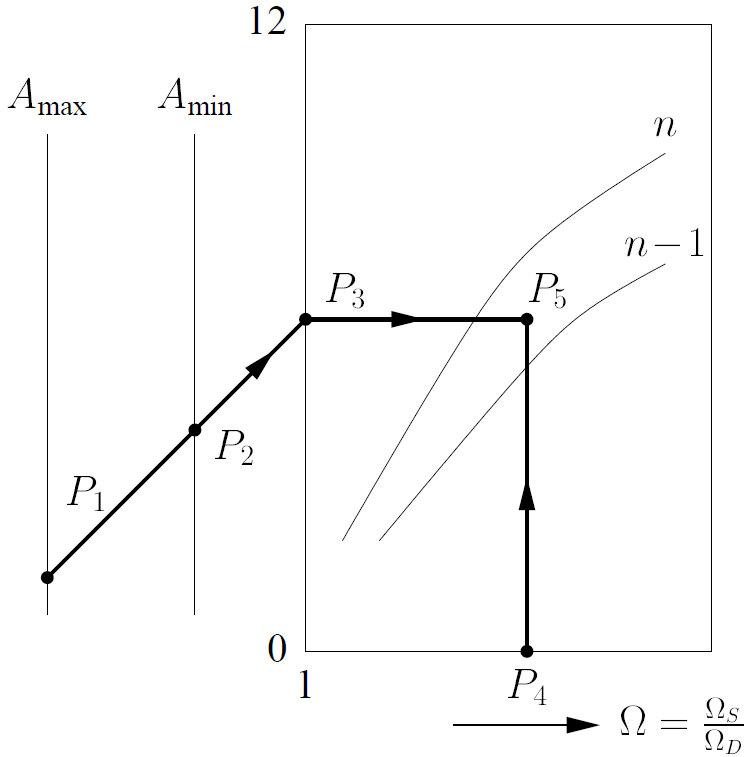
\includegraphics[width=\columnwidth]{images/filter_nomogramme.png}
\end{minipage}
\hfill
\begin{minipage}[c]{0.56\columnwidth}
    \begin{center}
        \textbf{\myul{Benutzung von Nomogrammen}}
    \end{center}
    
    \begin{enumerate}
        \item $P_1$: Verbindung von $A_{\rm max}$ zu $A_{\rm min}$
        \item $P_2$: Verlängerung von $P_1$ bis zum 'Diagramm-Rand'
        \item $P_3$: Horizontale Linie vom Rand in Diagramm hinein
        \item $P_4$: Bei $\Omega = \frac{\Omega_S}{\Omega_D} = \frac{\omega_S}{\omega_D} = \frac{f_S}{f_D}$ vertikale Linie ziehen
        \item $P_5$: Schnittpunkt: 'hochfahren' zur nächsten Kurve \textrightarrow\ Ordnung $n$ der Kurve ablesen
    \end{enumerate}
\end{minipage}


\subsection{LC-Filter: Entnormierung der Komponenten}
\label{Entnormierung Komponenten}

$$ \boxed{ L = \frac{L_{\rm norm}}{\omega_r} \cdot R_r}
\qquad \boxed{ C = \frac{C_{\rm norm}}{\omega_r \cdot R_r }}
\qquad \boxed{ R = R_{\rm norm} \cdot R_r } $$

\begin{center}
    \begin{tabular}{ll}
        $L_{\rm norm}$  & normierter Wert gemäss Skript, Anhang 7C \\
        $C_{\rm norm}$  & normierter Wert gemäss Skript, Anhang 7C \\
        $R_{\rm norm}$  & normierter Wert gemäss Skript, Anhang 7C \\
        $\omega_r$  & Frequenz, auf welche normiert wurde ($\omega_D$ oder $\omega_m$ gemäss \ref{Frequenznormierung}) \\
        $R_r$       & Tatsächlicher Wert von $R_2$ gemäss Topologie Skript S. 409
    \end{tabular}
\end{center}
    
